% 文档类
\documentclass[13pt]{ctexart}
% 设置页面
\usepackage{geometry}
% 插图片
\usepackage{graphicx}
% 设置标题 重命名为英文
\renewcommand{\figurename}{Figure}
\renewcommand{\tablename}{Table}
\renewcommand{\contentsname}{Contents}
% 设置摘要页缩减 
\usepackage{changepage}
% 便于修改字体
\usepackage{fontspec}
% 设置页眉页脚
\usepackage{fancyhdr}
% 清空页眉页脚
\pagestyle{fancy}
% 设置列表缩进
\usepackage[shortlabels]{enumitem}
% 设置修改默认的section标题大小
\usepackage{titlesec}
\titleformat*{\section}{\LARGE}
\titleformat*{\subsection}{\Large}
\titleformat*{\subsubsection}{\Large}
% 使用数学宏包
\usepackage{amsmath}
% 设置表格的列格式
\usepackage{array}
% 三线表宏包
\usepackage{booktabs}
% 设置产考文献不输出默认名
\usepackage{etoolbox}
\patchcmd{\thebibliography}{\section*{\refname}}{}{}{}
% 引入网站作为参考文献
\usepackage{url}
% 设置等宽的代码字体
\setmonofont{Courier New}
% 颜色
\usepackage{xcolor}
% 代码高亮方案宏包
\usepackage{listings}
\definecolor{CPPLight}  {HTML} {686868}
\definecolor{CPPSteel}  {HTML} {888888}
\definecolor{CPPDark}   {HTML} {262626}
\definecolor{CPPBlue}   {HTML} {4172A3}
\definecolor{CPPGreen}  {HTML} {487818}
\definecolor{CPPBrown}  {HTML} {A07040}
\definecolor{CPPRed}    {HTML} {AD4D3A}
\definecolor{CPPViolet} {HTML} {7040A0}
\definecolor{CPPGray}  {HTML} {B8B8B8}
\lstset{
	basicstyle=\ttfamily,
	breaklines=true,
	framextopmargin=50pt,
	frame=bottomline,
	columns=fixed,       
    %numbers=left,                                       % 在左侧显示行号
	frame=none,                                          % 不显示背景边框
	backgroundcolor=\color[RGB]{255,255,255},            % 设定背景颜色
	keywordstyle=\color[RGB]{40,40,255},                 % 设定关键字颜色
	numberstyle=\footnotesize\color{darkgray},           % 设定行号格式
	commentstyle=\itshape\color[RGB]{0,96,96},                % 设置代码注释的格式
	stringstyle=\slshape\color[RGB]{128,0,0},   % 设置字符串格式
	showstringspaces=false,                              % 不显示字符串中的空格
	language=python,                                     % 设置语言
	morekeywords={alignas,continute,friend,register,true,alignof,decltype,goto,
		reinterpret_cast,try,asm,defult,if,return,typedef,auto,delete,inline,short,
		typeid,bool,do,int,signed,typename,break,double,long,sizeof,union,case,
		dynamic_cast,mutable,static,unsigned,catch,else,namespace,static_assert,using,
		char,enum,new,static_cast,virtual,char16_t,char32_t,explict,noexcept,struct,
		void,export,nullptr,switch,volatile,class,extern,operator,template,wchar_t,
		const,false,private,this,while,constexpr,float,protected,thread_local,
		const_cast,for,public,throw,std},
	emph={map,set,multimap,multiset,unordered_map,unordered_set,numpy,graph,path,append,extend,
		unordered_multiset,unordered_multimap,vector,string,list,deque,
		array,stack,forwared_list,iostream,memory,shared_ptr,unique_ptr,
		random,bitset,ostream,istream,cout,cin,endl,move,default_random_engine,
		uniform_int_distribution,iterator,algorithm,functional,bing,numeric,},
	emphstyle=\color{CPPViolet}, 
}

\begin{document}
\newgeometry{top = 1cm, right = 2.54cm, left = 2.54cm, bottom = 2.54cm}
% 第一页的字体为times new roman
\setmainfont{Times New Roman}
\thispagestyle{empty}

\begin{table}[h]
    \quad { }  \begin{minipage}[t]{5.5cm}
        % arraystretch 是调节列高
        \begin{tabular}[t]{>{\centering\arraybackslash}b{10em}}
            \fontsize{12pt}{10pt}\selectfont \textbf{Problem Chosen}\\ [2pt]
            {\color{red} \fontsize{20pt}{10pt}\selectfont C}
        \end{tabular}
    \end{minipage}
    \begin{minipage}[t]{5.2cm}
        \begin{tabular}[t]{>{\centering\arraybackslash}p{10em}}
            \fontsize{12pt}{10pt}\selectfont \textbf{2022} \\ [-2pt]
            \fontsize{12pt}{10pt}\selectfont \textbf{MCM/ICM} \\ [-2pt]
            \fontsize{12pt}{10pt}\selectfont \textbf{Summary Sheet}
        \end{tabular}
    \end{minipage}
    \begin{minipage}[t]{3cm}
        \begin{tabular}[t]{>{\centering\arraybackslash}b{12em}}
            \fontsize{12pt}{10pt}\selectfont \textbf{Team Control Number} \\ [2pt]
            {\color{red} \fontsize{21pt}{10pt}\selectfont 2210390}
        \end{tabular}
    \end{minipage}
\end{table}
\vspace{-20pt}
\noindent{\rule{\textwidth}{0.5mm}}

% 标题
{\centering\fontsize{18}{16}\selectfont\textbf{{Portfolio Management Based on DDPG Algorithm of Deep Reinforcement Learning}}
% 摘要
\vspace{10pt} 

\fontsize{13}{10}\selectfont\textbf{{Summary}}\par}

\vspace{10pt}

% 正文字体 13 pt
\fontsize{13}{12.5}\selectfont

\begin{adjustwidth}{1cm}{1cm}
\indent { }{ }{ }{ }{ }{}

We propose a model using the deep reinforcement learning DDPG\cite{2019} algorithm to exploit the data characteristics of daily prices of volatile assets: gold and bitcoin over the last five years in order to decide whether traders should buy, sell or hold assets in their portfolios. The results show that using an initial \$1,000, from September 11, 2016 to September 10, 2021 according to the trading strategy given by the model, our portfolio [C,G,B] was able to reach a value of \$143,322.3 at the market price of that day.

We used the ARIMA model to predict the daily prices of the two volatile assets for the next year and applied our trading strategy, which eventually succeeded in maximizing the total return, verifying that our model produced the best strategy.

We also perform a sensitivity analysis on the transaction costs to demonstrate the robustness of our model. The results show that the transaction cost of both assets, being a fixed percentage of the transaction amount, can significantly affect the choice of trading strategy.


\vspace{15pt}
\textbf{key words} : deep reinforcement learning(DRL); deep deterministic policy gradient(DDPG); Autoregressive Integrated Moving Average(ARIMA); portfolio management
\end{adjustwidth} 

% 开始写 memo 信
% 更换字体为 palatino 也可以不换
\setmainfont{TeX Gyre Pagella}
\newpage
\newgeometry{left = 3.5cm, right = 3.5cm}
\thispagestyle{empty}

{\centering \fontsize{18pt}{14pt}\selectfont \textbf{MEMO}\par}

\noindent FROM: Team {} 2210390 , MCM C

\noindent To: The Traders

\noindent Date: February 18, 2022

\vspace{10pt}
\noindent
Dear Traders:

We would be honored to help you use past daily prices to determine whether you should buy, hold or sell assets in your investment group. We are writing this letter to report our findings.

We analyzed the daily prices of gold and bitcoin over a five-year period and applied deep reinforcement learning techniques to portfolio management using the Deep Deterministic Policy Gradient (DDPG) algorithm in deep reinforcement learning, which spreads risk by limiting the investment weights of individual assets and using a dropout algorithm ( Dropout), i.e., randomly dropping nodes when training the model, is used to solve the overfitting problem. The results show that the value of our deep reinforcement learning-based portfolio has increased significantly by 1400\% over a five-year period, demonstrating the effectiveness of our approach. Further experiments show that our portfolio performs better when the data used for training is closer to the test data.  

In addition, since commissions are not a fixed percentage of the transaction amount in real market trading, we perform a sensitivity analysis of the transaction costs and recommend that you change your trading strategy according to the fluctuation of the costs in order to maximize the total return.


We believe that our model is useful for trading in the future. You are welcome to contact us at any time for further cooperation.

% 信多出一页,清理页眉页脚
\thispagestyle{empty}
% 信的结尾
{\raggedleft
Sincerely yours

MCM C Team 2210390\par
}

% 目录页
\newpage
\thispagestyle{empty}
\tableofcontents
\newpage
% 目录页后面是第一页
\setcounter{page}{1}

% 开始写正文
% 设置正文的页边距
\newgeometry{top=3cm, left=3.5cm, right=3.5cm}
% 设置正文的页眉页脚
\fancyhf{}
\fancyhead[C]{ }
% 此处修改右上角页码
\fancyhead[R]{Page \thepage\ of 25}
%\fancyhead[R]{Page \thepage\ of 15}
\fancyhead[L]{Team \# 2210390}
\fancyfoot[C]{\bfseries\thepage}
\textbf{\section{Introduction}}
\textbf{\subsection{Background of the problem}}
Market traders frequently buy and sell unstable assets (e.g. Bitcoin, gold, etc.), constantly reallocating their capital to different financial products with the aim of reducing transaction costs and increasing investment returns, while curbing risk.

However, financial markets are unpredictable, with new policies, changes in the social and natural environment, scientific and technological developments, and even psychological factors of important investment groups causing changes in the market, making it very difficult to accurately predict the rise or fall of market prices.

To obtain stable profits, investors need to accurately grasp the overall laws of the market and develop a scientific and clear quantitative trading strategy to determine the time, object and quantity of each transaction. Traditional portfolio management methods include "follow the winner", "pattern matching" and "meta-learning".

In recent years, deep learning has been successfully applied in various financial fields, including quantitative trading. Deep learning can extract imperceptible features from complex financial markets to assist firms and institutions in developing scientific quantitative trading strategies. And automated trading intelligences in reinforcement learning are able to buy, sell or hold assets as actions and seek optimal trading strategies in interaction with the market environment.
\textbf{\subsection{Restatement of the Problem}}
Between September 11, 2016 and September 10, 2021, we are asked to trade bitcoin and gold with an initial \$1000.

\begin{itemize}
	\item Design a model that gives a daily trading strategy based on the daily gold and bitcoin trading prices on that day. 
	\item Calculate the final value of the investment on September 10, 2021.
	\item Prove that our model provides the best trading strategy.
	\item Perform a sensitivity analysis to determine how sensitive the strategy is to the cost of trading.
\end{itemize}
\textbf{\subsection{Our Works}}


\begin{itemize}
	\item First, we apply deep reinforcement learning techniques to portfolio management, using the deep deterministic strategy gradient DDPG algorithm in deep reinforcement learning to build the model.
	\item Then, we solve the overfitting problem by limiting the investment weights of individual assets to diversify the risk, and by using a discard algorithm, i.e., randomly discarding nodes when training the model.
	\item Next, we use the ARIMA model to predict daily prices for the next year, verifying that the trading strategy generated by our model is optimal.
	\item Finally, we analyze the sensitivity of the trading strategy to cost, and adjust the trading strategy appropriately according to the fluctuation of the commission ratio.
\end{itemize}
\textbf{\section{Assumptions and Notations}}
\vspace*{-10pt}
\textbf{\subsection{Assumptions}}
\begin{itemize}[itemsep=0.3ex, leftmargin=1.2cm]
	\item[1.] We consider only backtest trading, i.e., we only know the current and historical market state at a given moment before making a trading decision, and not the future market condition.
	\item[2.] The money trading operations we perform as individual traders do not have any impact on the overall market up or down situation.
	\item[3.] The daily value of gold and bitcoin is constant and the price per trade is the same as the value in the tables LBMA-GOLD.csv and BCHAIN-MKPRU.csv.
	\item[4.] We can complete any transaction at the moment of market opening, i.e. there is no inability to buy or sell.
	\item[5.] The cost of a transaction is a fixed percentage of the day's trading volume.
	\item[6.] We can buy any amount of gold and bitcoin according to the optimal allocation weighting, and the number of purchases can be a non-integer number.
\end{itemize}
\textbf{\subsection{Notations}}
Here are all the notations and their meanings in this paper.
\begin{table}[h]
	\centering
	\vspace{3pt}
	\begin{tabular}{>{\centering\arraybackslash}p{5em}>{\centering\arraybackslash}p{30em}}
	\toprule % 绘制第一条线
	Symbol & Meaning \\ \midrule
	$t$ & Time \\
	$a$ & Action\\
	$s$ & State\\
	$y_t$ & The investment return of each asset of the portfolio expressed as a vector\\
	$V_t$ & represents the closing price of the corresponding asset in the portfolio at time  $t$ \\ 
	$p_t$ & Total value of the portfolio at time $t$ minus transaction costs \\
	$r_t$ & The return of the portfolio at time $t$ \\ 
	$w_t$ & denotes the weight of each asset of the portfolio at the corresponding moment \\
	$\pi$ & Strategy  \\
	$γq_t$ & Network Parameters \\
	\bottomrule
	\end{tabular}
\end{table}

\textbf{\section{Model Construction}}
\textbf{\subsection{Deep learning}}
Deep learning is a general framework for learning representations using a multilayer nonlinear transformation processing network structure. Thanks to the improvement of computer performance, deep learning has greatly improved the effectiveness of artificial neural network methods and is an important method in the field of artificial intelligence in recent years.

Traditional artificial neural networks are not suitable for deep networks because they are prone to local optimal solutions or overfitting problems as the number of layers of neural networks increases.This makes learning time-consuming and labor-intensive.

The concept of deep learning was proposed by Hinton et al. at the University of Toronto, Canada, in 2006, based on the unsupervised layer-by-layer pre-training and supervised tuning algorithms of the Deep Belief Network (DBN), which can automatically learn data features and effectively optimize the learning results, solving the problem that the deep neural network structure is prone to local optimal solutions. The problem of local optimal solution of deep neural network structure and the problem of manual design of data features were solved. Later, Hinton proposed the Dropout method to solve the overfitting problem of neural networks. After that, deep learning developed rapidly and was widely used in speech, image, medical and financial fields. The common network structures of deep learning include deep neural network DNN (Deep Neural Networks), deep belief network DBN, convolutional neural network CNN, recurrent neural network RNN, LSTM, etc.
\textbf{\subsection{Reinforcement learning}}
Reinforcement learning, also known as augmented learning or reactive learning. The main idea of reinforcement learning is that an intelligent body interacts with its environment through trial and error, and uses evaluative feedback signals to optimize its decisions. When an action of an intelligent body leads to a positive reward or reward from the environment, which is the reinforcement signal, the tendency of the intelligent body to produce this action in the future will be strengthened.

Conversely, the tendency to produce this action will be weakened. There are four main elements of reinforcement learning, namely, strategy, reward, action, and environment. The goal of reinforcement learning is to learn a strategy so that the action chosen by the intelligence receives the maximum reward from the environment. The payoff can be calculated as a function, also known as the payoff function. In order to measure the long-term effect of reinforcement learning, a value function (the

In order to measure the long-term effects of reinforcement learning, the value function is often used instead of the payoff function to measure not only the immediate payoff of an action, but also the cumulative payoff of a series of possible subsequent states from that state onward.

Classical reinforcement learning methods are often unable to solve the problem of high spatial dimensionality of states and actions, and an effective solution is to use function approximation, which represents the value function or strategy as a function. Commonly used approximation functions include linear functions, kernel functions, and neural networks. The most successful function approximation method in recent years is to use deep neural network as a nonlinear approximation function for reinforcement learning, which combines deep learning and reinforcement learning, that is, deep reinforcement learning. Deep reinforcement learning was first proposed by DeepMind team in 2015, and then developed and applied to AlphaGo, which defeated the human Go champion, and AlphaGo Zero, which was even stronger. The deep deterministic policy gradient method, DDPG algorithm, proposed by DeepMind team in 2016, solves the problem of reinforcement learning in continuous action space. In DDPG algorithm, the strategies are parametrized and the parameters of the deep neural network are directly optimized by the strategy gradient method.

\textbf{\subsection{Deep deterministic policy gradient}}
The full name of DDPG\cite{2020Deep} is Deep Deterministic Policy Gradient, which means Deep Deterministic Policy Gradient. From the name of DDPG, it is composed of D(Deep) + D(Deterministic ) + PG(Policy Gradient). Then its features can also be broken down in this way.
%无序列表
\begin{itemize}
	\item The motivation of DDPG is actually to allow DQN to be extended to a continuous action space.
	\item DDPG borrows two techniques from DQN: experience replay and fixed Q-network.
	\item DDPG uses a policy network to output deterministic actions directly.
	\item DDPG uses the Actor-Critic architecture.
\end{itemize} 

DDPG is an extended version of DQN that can be extended to the control space of continuous actions. Therefore it adds a layer of policy network on top of DQN for outputting action values.DDPG needs to learn the Q network while learning the policy network.

DDPG has 4 networks, Actor current network, Actor target network, Critic current network, and Critic target network.
\begin{itemize}
	\item Actor current network: responsible for iterative update of policy network parameters θ, responsible for selecting current action A based on current state S, used to interact with environment to generate S′,R.
	\item Actor target network: responsible for selecting the optimal next A′ based on the next state S′ sampled in the experience replay pool. The network parameter θ′ is periodically copied from θ.
	\item Critic Current Network: Responsible for iterative update of the value network parameter w. Responsible for computing the current Q value Q(S,A,w) responsible for computing the current Q value. Target Q-value yi=R+γQ′(S′,A′,w′)
	\item Critic target network: responsible for computing the Q′(S′,A′,w′) part of the target Q-value. The network parameters w′ are periodically copied from w.
\end{itemize}

The replication of DDPG from the current network to the target network is different from DQN, which directly replicates the parameters of the current Q network to the target Q network, i.e., w′=w. DDPG does not use this hard update here, but uses a soft update, i.e., the parameters are updated only a little bit at a time, i.e.
%插入公式
\begin{equation}
	\begin{array}{c}
		w \prime \leftarrow \tau w+(1-\tau) w \prime \\
		\theta \prime \leftarrow \tau \theta+(1-\tau) \theta \prime
		\end{array}
\end{equation}
\textbf{\section{Model Simulation and Analysis}}
\textbf{\subsection{Model Representation}}
\textbf{\subsubsection{Asset composition of the portfolio}}
The portfolio in this paper consists of 2+1 financial assets, including 2 risky assets and one currency (USD). The total weight of the portfolio is set to 1. If only risky assets are included in the portfolio, investors will have to hold all risky assets when the market is underperforming, which will reduce the return and increase the risk. By including currency as an asset in the portfolio, it is possible to hold only currency when the market is underperforming, which is equivalent to not holding risky assets.
\textbf{\subsubsection{Portfolio asset weights and returns}}
Let $ y_t $ be the investment return of each asset of the portfolio on the interval [t - 1, t] expressed as a vector, which is referred to as the return vector as follows:
%插入公式
\begin{equation}
	y_{t}=\left[1, \frac{V_{g, t, \text { close }}}{V_{g, t-1, \text { close }}}, \frac{V_{b, t, \text { close }}}{V_{b, t-1, \text { close }}}\right ] 
\end{equation}

The first component of the vector represents the yield of the currency, which is 1 because there is no additional gain from just holding the currency, and the value of the currency remains constant from start to finish. The vector of $ V_{g, t, \text { close }} $ is denotes the closing price of gold in the portfolio at time t; $ V_{b, t, \text { close }} $ is denotes the closing price of Bitcoin in the portfolio at time t.Where i = 1, 2, ..., N, thus $ \frac{V_{i, t, \text { close }}}{V_{i, t-1, \text { close }}} $ denoting the return on investment of i assets over the interval [t - 1, t].

Let $ p_t $ be the total value of the portfolio at time t after subtracting transaction costs, $ p_{t-1} $ be the total value of the portfolio at time t - 1 after subtracting transaction costs, $ p_0 $ be the initial value of the portfolio, and $ p'_t $ be the total value of the portfolio at time t before subtracting transaction costs. Let $ r_t $ be the return of the portfolio at time t, i.e.
\begin{equation}
	r_{t}=\frac{p_{t}}{p_{t-1}}
\end{equation}

Let $ R_t $ be the cumulative total return of the portfolio at time t, i.e.:
\begin{equation}
	\mathrm{R}_{\mathrm{t}}=\frac{\mathrm{p}_{\mathrm{t}}}{\mathrm{p}_{0}}
\end{equation}

The weight of each asset in the portfolio at [t - 1, t] is denoted by $ w_t $ and is referred to as the weight vector, as follows:
\begin{equation}
	W_{1}=\left[\begin{array}{lll}W_{1 t}, & W_{g t}, & W_{b t}\end{array}\right] 
\end{equation}

Thus Ease of Knowing:
\begin{equation}
\frac{p_{t}^{\prime}}{p_{t-1}}=w_{t} \cdot y_{t}
\end{equation}

\textbf{\subsection{DDPG algorithm structure}}
The basic elements of reinforcement learning include an intelligent agent, an environment, a state s, a policy π, an action a, and a reward r. The agent perceives the current state $ s_t $ from the environment, selects an action $ a_t $ according to the policy π, acts on the environment, and obtains a reward $ r_t $, which is converted to the next state $ s_{t + 1} $. Since the reward $ r_t $ only reflects the reward of the current action and state, but not the impact on the future reward, a value function v is also introduced. The value function v is introduced, which contains the current returns and the estimated discounted (denoted by γ) future returns. Deep reinforcement learning methods use deep neural networks to learn strategies in the continuous action space, which are parametrically represented, and the output is the action.

The DDPG algorithm\cite{2017A} adopts the reinforcement learning Actor-Critic architecture, which consists of 4 neural networks: 2 structurally identical Actor strategy networks, Actor-online network and Actor-arget network respectively; 2 structurally identical Critic evaluation networks, Critic-online network and Critic -target networks. The Actor-target and Critic-target networks are mainly used to generate the training data set, while the Actor-online and Critic-online networks are mainly used to train and optimize the network parameters. Compared with other neural networks, LSTM networks are more suitable for time series data prediction, so LSTM is used in this paper.

The two Actor strategy networks are composed of a long and short term memory network layer LSTM, a fully connected network layer (FC) and a softmax layer, where the activation function of the fully connected network layer is a linear correction function (ReLU). The network input is the state, i.e., the asset price $ s_t $, and the output is the buy and sell action $ a_t $.

Both Critic evaluation networks are composed of an LSTM network layer, an FC fully connected network layer (input is asset price $ s_t $) and an FC fully connected network layer (input is action $ a_t $), and the last two FCs are summed to another FC fully connected network layer. The network inputs are the asset price $ s_t $ and the buy and sell action $ a_t $, while the output is the estimated future discounted return $ γq_{t + 1} $.

The structure of the DDPG algorithm is shown in Figure 1.
\begin{figure}[h]
	\centering
	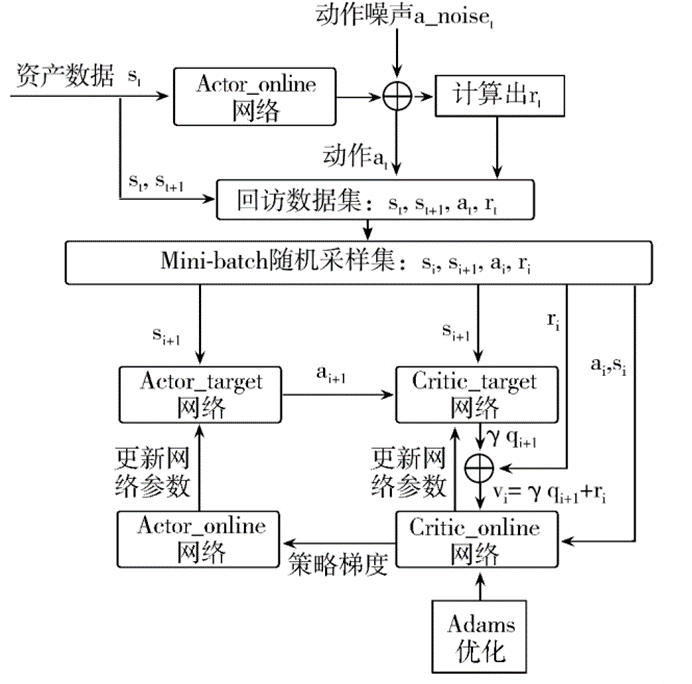
\includegraphics[width=0.8\textwidth]{img/img1.png}
	\caption{DDPG architecture}
	\label{fig:DDPG_architecture}
\end{figure}

The DDPG algorithm is described in the following steps:
%有序列表
\begin{enumerate}
	\item	The Actor-online network generates the playback dataset: the initial action is output according to the asset price  $ s_t $ , and the action  $ a_t $  is output with the random noise a-noiset, and the immediate return rt is calculated, i.e., the current return; the transition to the next state, i.e., the asset price  $ s_{t + 1} $  at the next moment.The training data set, also called the playback data set, consists of (  $ s_t $ ,  $ a_t $ ,  $ r_t $ ,  $ s_{t + 1} $ ).
	\item	Mini-batch sampling is performed on the playback data set, i.e., the same number of random and consecutive samples are sampled each time as the training data for the network. The set of data in a single Mini-batch is represented by ( $ s_i $ ,  $ a_i $ ,  $ r_i $ ,  $ s_{i + 1} $ ).
	\item 	Estimate the value function vi using the Mini-batch sampled data.  $ a_{i + 1} $  is calculated by the Actor-target network,  $ γq_{i + 1} $  is calculated by the Critic-target network, and finally the value function  $ v_i = r_i + γq_{i + 1} $  is calculated.
	\item 	The Critic-online network is trained with the Mini-batch sampled data and the calculated value function  $ v_i $ , and optimized by Adams (AdaptiveMoment Estimation) method, while the Critic-online network optimizes the Actor-online network by the policy gradient.
	\item 	Finally, the parameters of the Actor-target network and the Critic-target network are updated by the Critic-online network and the Actor-online network, respectively.
\end{enumerate}
\textbf{\subsection{Problems encountered and solutions}}
The computer operating system is Windows 11, the running environment is Tensorflow 1.4, and the programming language Python 3.7 is used. In the actual training of the network, we mainly found the problems of overfitting and unreasonable distribution of asset weights, and we analyze the causes and solutions below.
%有序列表
\begin{enumerate}
	\item In the process of algorithm implementation, the neural network is prone to good results in training and poor performance in testing, which means that the network is too dependent on the training data set, and therefore cannot effectively handle new data when they appear, that is, the phenomenon of overfitting. In order to solve this problem, the following measures are taken: add Dropout option to all LSTM networks; appropriately reduce the number of samples of the data set (Max Step); change the window length of the input asset data (Window Length), "Window Length" is set in the trading process The "Window Length" is the number of days of historical data set in the trading process, which is used to calculate the current optimal weighting.
	\item Since reinforcement learning is based on a Markovian decision process, i.e., future returns are considered to be independent of past states, but only related to current and future states. Since the risk (i.e., variance) of a portfolio needs to be calculated from historical data, minimizing the risk of a portfolio as an optimization objective will make the future return related to the past state. Therefore, the approach used in this paper takes the maximization of the value function v (i.e., current return plus future discounted return) as the only optimization objective, and thus cannot simultaneously minimize risk. However, the original weights can be further processed in order to properly diversify the asset weights in the portfolio to optimize the return and reduce the risk without affecting the performance of the portfolio.
\end{enumerate}
\textbf{\section{Strengths and Weaknesses}}
Based on the modeling process, we make some comments on our model as listed below.
\textbf{\subsection{Strengths}}
\begin{itemize}
	\item a final total return on investment of 14 times the initial capital.
	\item that the reinforcement learning algorithm enables the trading strategy to adapt well to new environments.
	\item deep neural networks predict the rise and fall of financial asset prices in the short term with a high accuracy rate.
\end{itemize}
\textbf{\subsection{Weaknesses}}
\begin{itemize}
	\item less data, prone to overfitting problems, resulting in too much concentration of asset weights. 
	\item failed to consider the impact of its own transactions on market prices.
	\item only two assets have been experimented, for other markets need to be further explored.
\end{itemize}
\textbf{\section{Sensitivity Analysis}}
The ARIMA model can be expressed by the following equation
\begin{equation}
	\left(1-\sum_{i=1}^{p} \varphi_{i} L^{i}\right)(1-L)^{d} X_{t}=\delta+\left(1+\sum_{i=1}^{q} \theta_{i} L^{i}\right) \varepsilon_{t}
\end{equation}

First, we use the model and historical daily prices to forecast volatile assets with a gradient of transaction cost ratios against six groups set at 0.5%, 1%, 1.5%, 2%, 2.5%, and 3%.

The results show that trading strategies will tend to abstain from buying when the cost is too high until the increase in return is greater than the increase in cost.
%插入图片
\begin{figure}[h]
	\centering
	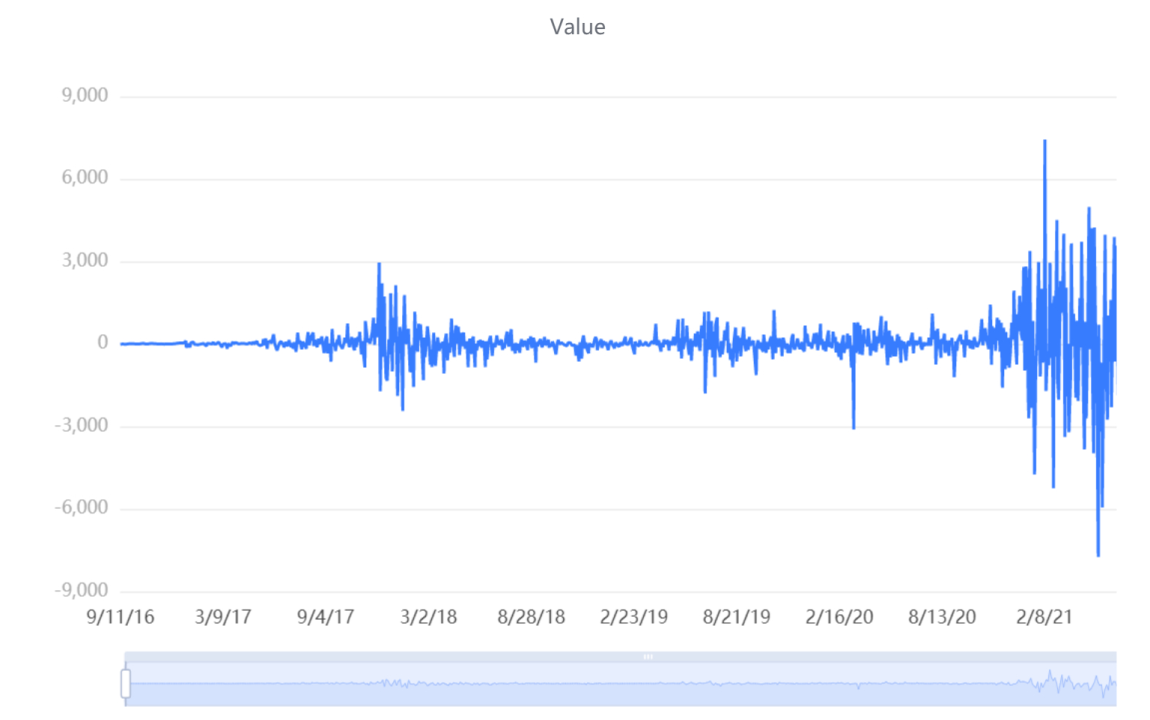
\includegraphics[width=0.8\textwidth]{img/img2.png}
	\caption{Best Difference Sequence Chart}
	\label{fig:Sensitivity_Analysis}
\end{figure}

We then compared the results with policy gradient. The model with the policy gra⁃dient algorithm obtained 12,435 RMB at the end of the test, with an annual return of 17.53%; the model with the policy gra⁃dient algorithm obtained 10,580 RMB at the end of the test, with an annual return of 4.18%; the method of investing all the money in a single asset and holding it until the end of the test obtained an average of 11,457 RMB at the end of the test, with an annual return of at the end of the test with an average return of RMB 11,457 and an annual return of 10.49%.

Analyzing the results, we can see that our model has the highest annual return.
\begin{figure}
	\centering
	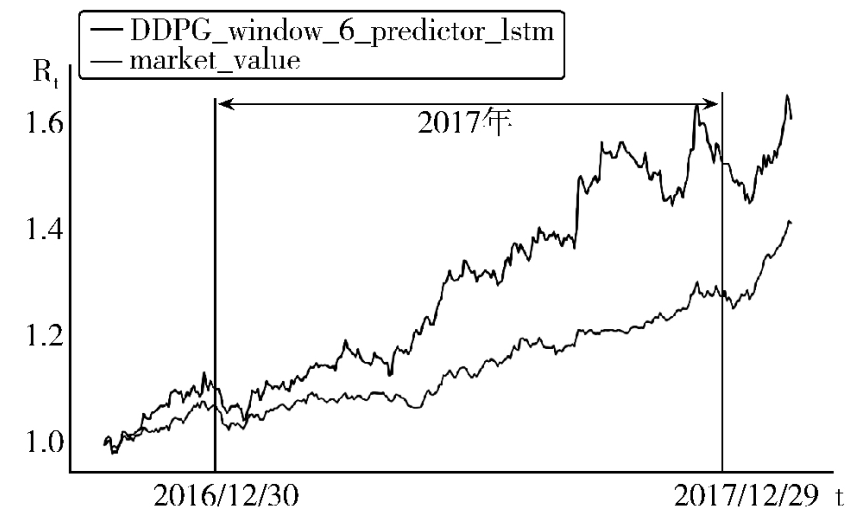
\includegraphics[width=0.8\textwidth]{img/img3.png}
	\caption{Comparison of our portfolio with the control group}
	\label{fig:Sensitivity_Analysis}
\end{figure}
\textbf{\section{Conclusion}}
Since there is no application of deep reinforcement learning technology in portfolio management, this paper improves the DDPG algorithm of deep reinforcement learning for the first time to enable its application in portfolio management by limiting the investment weights to diversify the risk and using the discard algorithm to solve the overfitting problem. In this paper, two unstable assets are used as risky assets in the portfolio for experiments. The experimental results show that the performance of the portfolio constructed by this method is much better than that of other control groups, which demonstrates the effectiveness of this method.

However, some assumptions are made for the sake of simplification, such as the assumption that the trading capital is small enough not to affect the behavior of other investors in the market and the price of financial assets, but when the users of this method are institutional investors or individual investors with large capital, they need to consider the impact of their own trading on the market price, so it is necessary to conduct more in-depth research.

In addition, the algorithm can be applied to portfolios to maximize rewards while maximizing entropy, ensuring stability and explorability. The model proposed in this paper takes raw market data and historical prices as input and directly outputs the weight vector of financial assets in the portfolio. The method proposed in this paper, does not rely on any financial theory and is therefore highly scalable. After analysis, we have achieved satisfactory results in terms of returns, annual returns.

The limitation of the work in this paper is that it is not possible to use historical data to fully simulate real online transactions. Future improvements can be made in terms of how to selectively and purposefully pick quality investments and add financial market information.
% 因为不输出此部分到目录 \addcontentsline{}{}{}是添加此标题到目录 
\newpage
\textbf{\section*{References}\addcontentsline{toc}{section}{References}}
\fancyhf{}
\fancyhead[R]{ }
\fancyhead[L]{ }
\bibliography{books}
\Large
\bibliographystyle{IEEEtran}

\newpage
\textbf{\section*{Appendices}\addcontentsline{toc}{section}{Appendices for Code and Data}} 
\fontsize{13pt}{12.5pt}\selectfont
Here is Code we used in our model, which python is the main development language.
\vspace{7pt}
\textbf{\subsection*{Appendices A: An automated trading robot training environment built on deep reinforcement learning}}
\noindent{\rule{\textwidth}{0.2mm}}
\vspace{-18pt} 
\fontsize{13pt}{12.5pt}\selectfont
{
	\lstinputlisting[language=python]{envs.py}
}
\vspace{-15pt}
\noindent{\rule{\textwidth}{0.2mm}}


\end{document}